\documentclass{article}
\usepackage[utf8]{inputenc}
\usepackage{graphicx}
\usepackage{parskip}
\usepackage{textcomp}
\usepackage{hyperref}
\hypersetup{
    colorlinks=true,
    linkcolor=blue,
    filecolor=magenta,      
    urlcolor=cyan,
}
\usepackage{listings}
\lstset{language=C,
                basicstyle=\ttfamily,
                keywordstyle=\color{blue}\ttfamily,
                stringstyle=\color{red}\ttfamily,
                commentstyle=\color{green}\ttfamily,
                morecomment=[l][\color{magenta}]{\#}
}

\title{The Breakout Game}
\author{By \\ Umang Deshpande and Akshay Hegde}
\date{June 2017}

\begin{document}
\maketitle

\section{Objectives}
\begin{itemize}
    \item Understanding RTOS and Statechart Principles.
    \item Design and Development of the Breakout game.
    \item Implementation of the game on the console.
\end{itemize}

\section{Prerequisites}
\begin{itemize}
    \item Basics of RTOS, familiarization with tasks, semaphores and task scheduling.
    \item Drawing up of a statechart from the game design statement (Please refer to the Bomb Timer example in the Resources Section).
    \item Implementation of visual statechart in code using switch case construct (Please refer to the link given \href{https://stackoverflow.com/questions/31100824/finite-state-machine-in-c}{here}).
    \item Creation of GLCD graphic for game objects(Please refer to the Mikroelektronika GLCD Font Creator Example in the Resources Section).
\end{itemize}

\section{Game Design Statement}
\qquad The overall objective is to design the classic Breakout Game for the Tiva C Game Console, using the onboard peripherals.
The breakout game has a rectangular paddle at the bottom of the screen off which a moving ball ricochets off. At the top of the screen, it consists of rows of bricks. The victory condition is to clear the row of bricks, by hitting it with the ball. Our implementation of the game is to have 5 types of bricks:
\begin{itemize}
  \item \textit{HARD} brick - Takes 3 hits to disappear.
  \item \textit{MEDIUM} brick - Takes 2 hits to disappear.
  \item \textit{EASY} brick - Takes 1 hit to disappear.
  \item \textit{MAGIC1} brick - Delivers a hit to all surrounding bricks.
  \item \textit{MAGIC2} brick - Increases paddle size for 10 seconds.
\end{itemize}
There are 3 difficulty levels:
\begin{itemize}
  \item \textit{EASY} - 3 lives, higher proportion of EASY bricks.
  \item \textit{MEDIUM} - 2 lives, higher proportion of MEDIUM bricks.
  \item \textit{HARD} - 1 life, higher proportion of HARD bricks.
\end{itemize}
Implicit above is an implementation of a life system(allowed number of retries for the player). There are three speeds for the ball:
\begin{itemize}
  \item \textit{SLOW} - Ball moves slowly.
  \item \textit{MEDIUM} - Ball moves at an average speed.
  \item \textit{FAST} - Ball moves very fast.
\end{itemize}
Additionally, the game has the following screens:
\begin{itemize}
  \item Entry Cutscene
  \item Menu Screen
  \item Instructions Screen(Accessible from the menu)
  \item Settings Screen(Accessible from the menu)
  \item Gameplay Screen
  \item Victory Screen
  \item Game Over Screen
\end{itemize}

\section{Relevant Theory}
\subsection{Statechart Solution}
\qquad Since the game has several active components at the same time, it runs several parallel state machines each of which may or may not be independent of the other. The different state machines are as follows:
\begin{center}
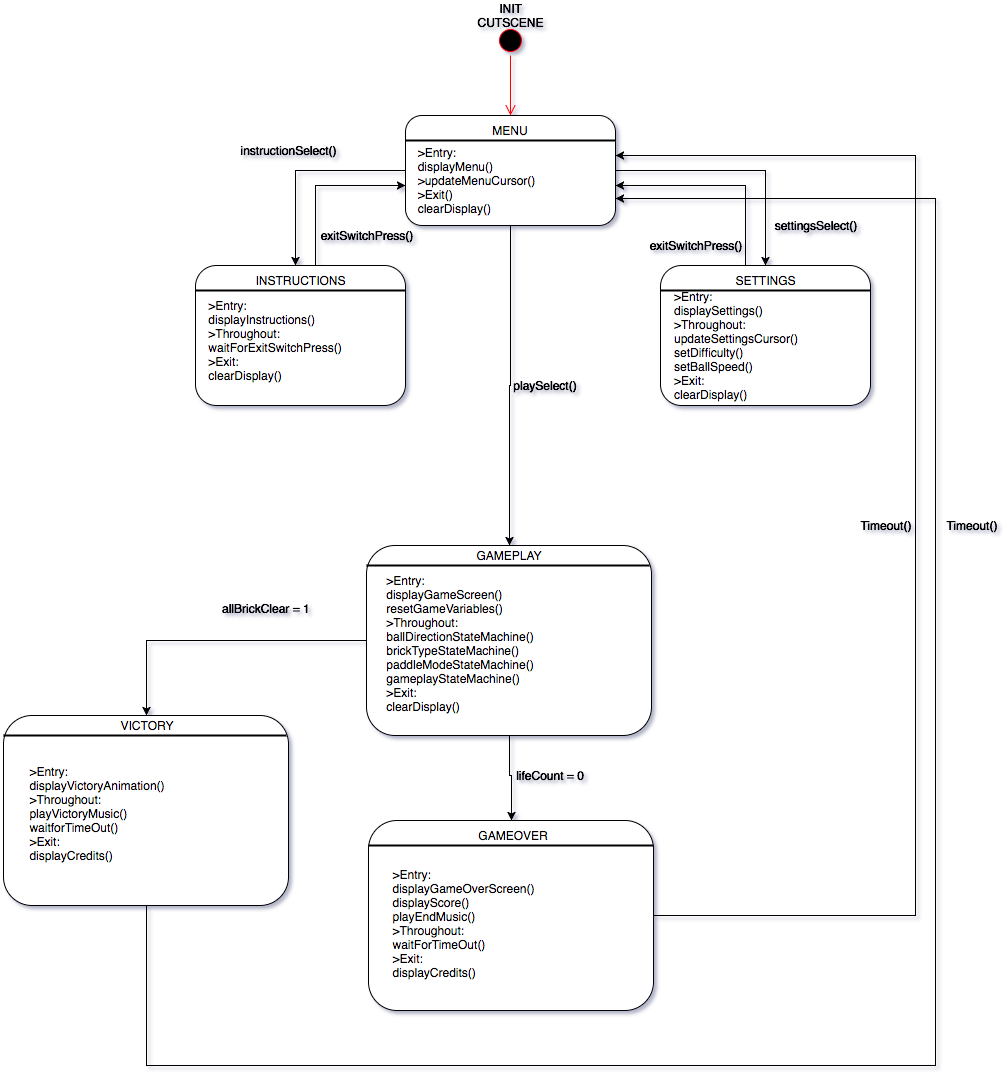
\includegraphics[width=14cm, height=18cm]{Images/gameStateMachine} \\
\caption{Fig (a): Game Screens State Machine} \\
\end{center}
\newpage
\qquad The overall states in which the game exists is as shown in Fig (a). A brief explanation of each state is as follows:
\begin{itemize}
  \item \textbf{MENU} State: \\ \qquad This acts as the GUI for the user, and follows the initial cutscene(The Cutscene displays the cutscene graphic while playing Music).  The Menu Screen is then displayed, and switch presses are used to move the cursor. 
  \\ \textit{RIGHT} Switch press is used for selection.
  \\ \textit{UP} Switch press is to move cursor up.
  \\ \textit{DOWN} Switch press is to move cursor down.
  \\ A screenshot of a sample \textit{MENU} state is as shown
  \begin{center}
  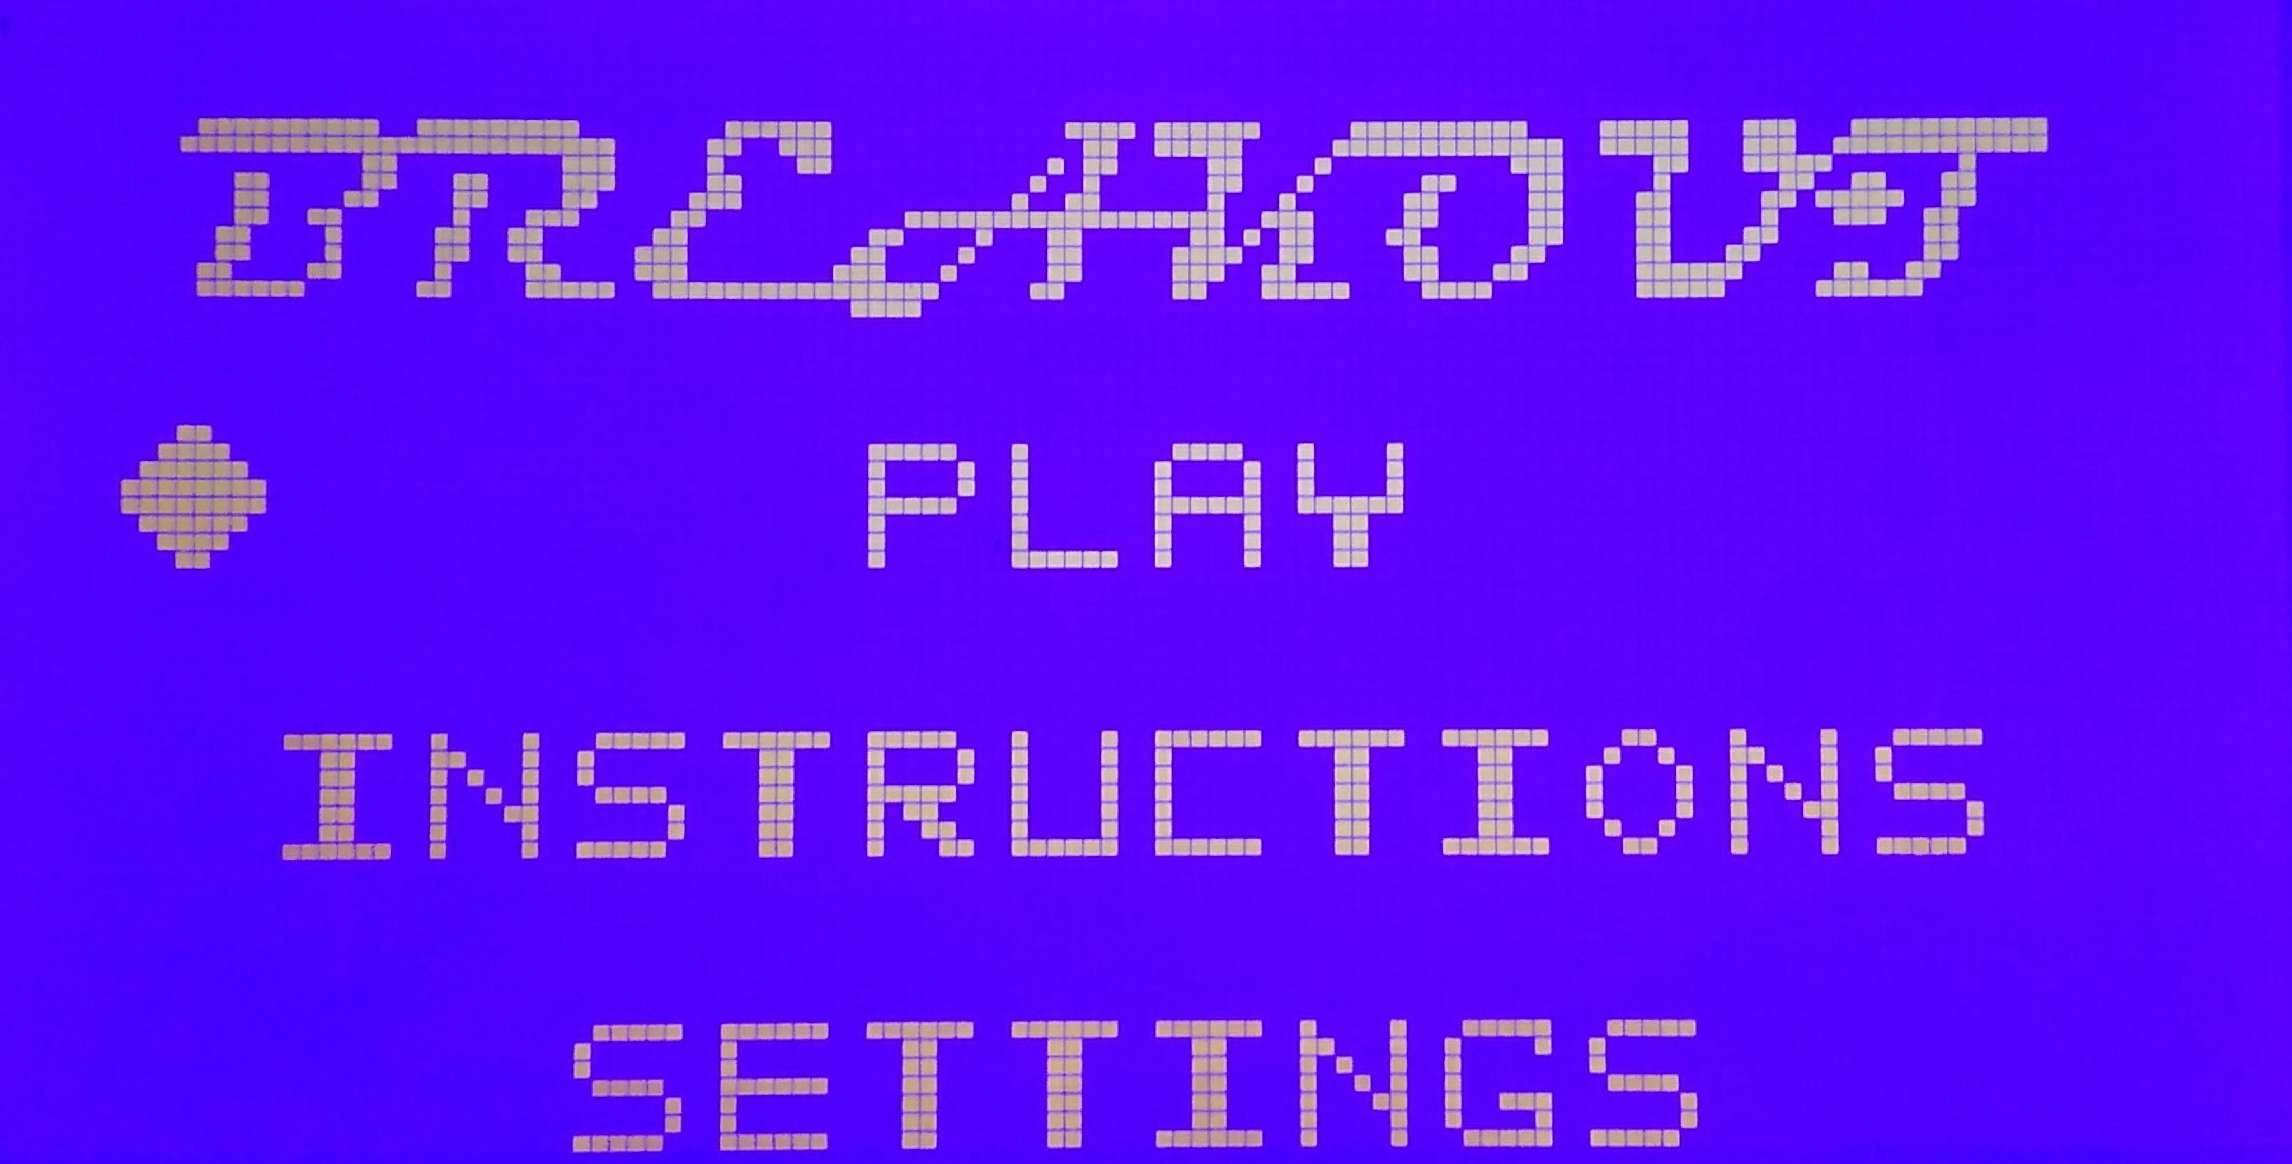
\includegraphics[width=10cm, height = 5cm]{Images/menuScreen} \\
  {\small Fig (b): Menu Screen} \\
  \end{center}
  \item \textbf{INSTRUCTIONS} State: \\ \qquad This displays instructions of gameplay for the user.
  \textit{LEFT} Switch Press = Back.
  \\ A sample \textit{INSTRUCTIONS} screen:
    \begin{center}
  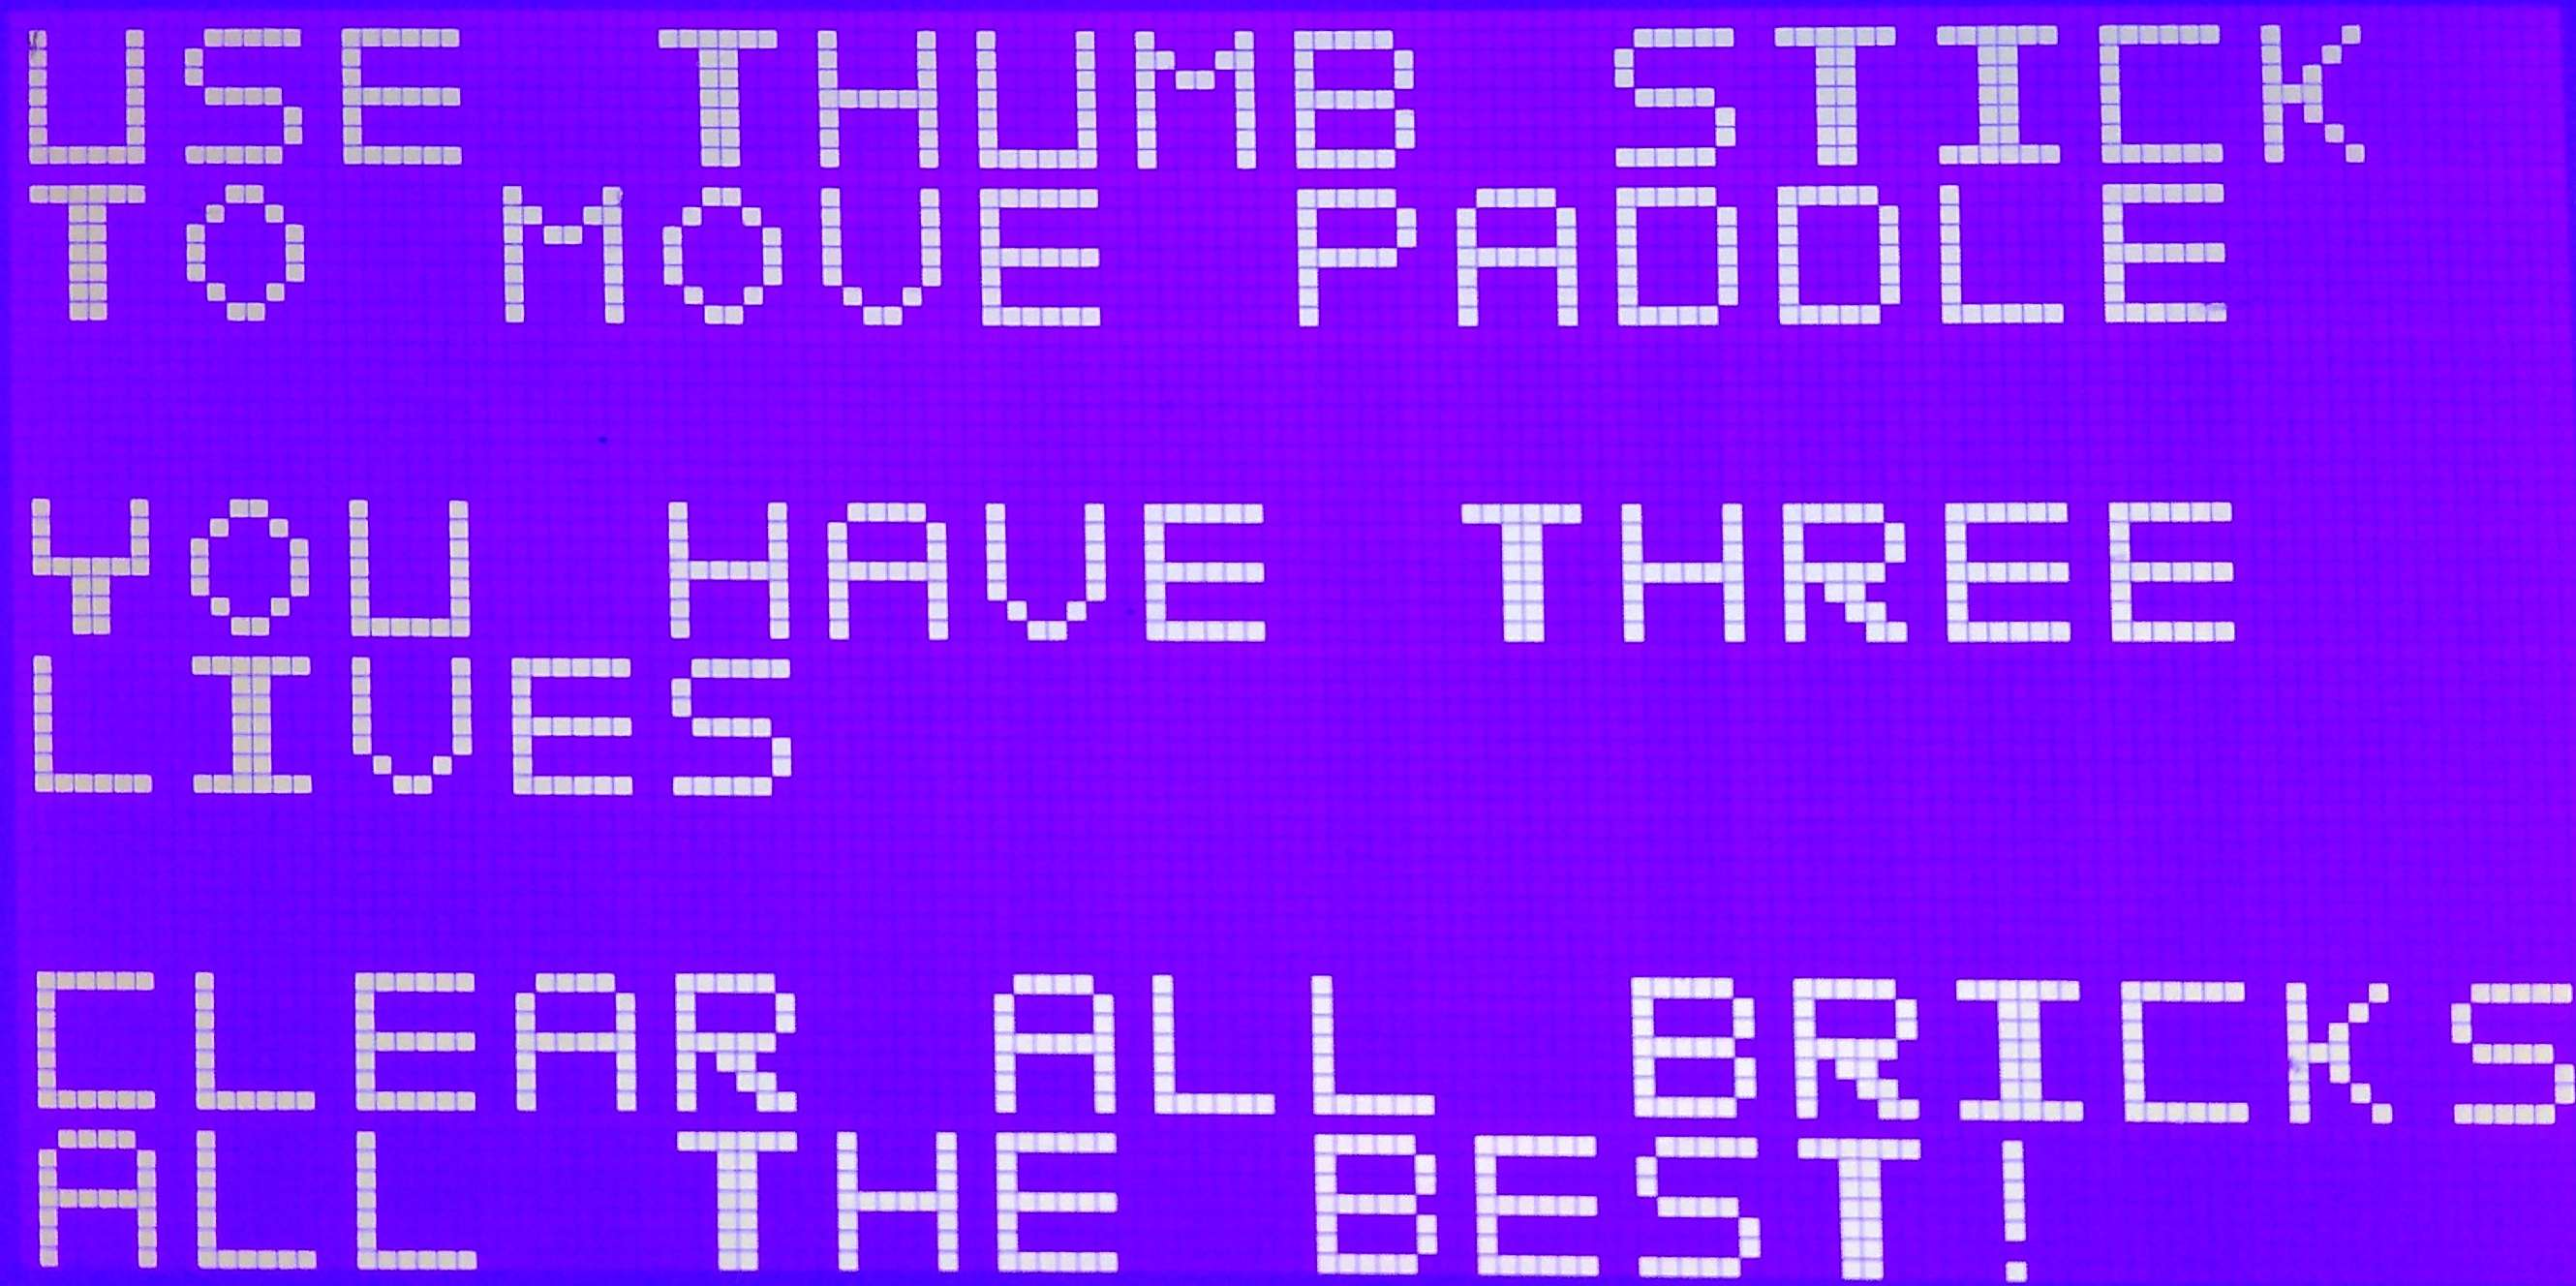
\includegraphics[width=10cm, height = 5cm]{Images/instructionsScreen} \\
  {\small Fig (c): Instructions Screen} \\
  \end{center}
  \item \textbf{SETTINGS} State: \\ \qquad This allows for change of difficulty and ball speed settings for the player.
  \\ \textit{UP} Switch moves cursor up, and at topmost position, acts as back Switch.
  \\ \textit{DOWN} Switch moves cursor down, and at bottommost position, acts as back Switch.
  \\ \textit{LEFT} selects easiest setting, RIGHT selects toughest setting, HAT selects medium setting.
  \begin{center}
  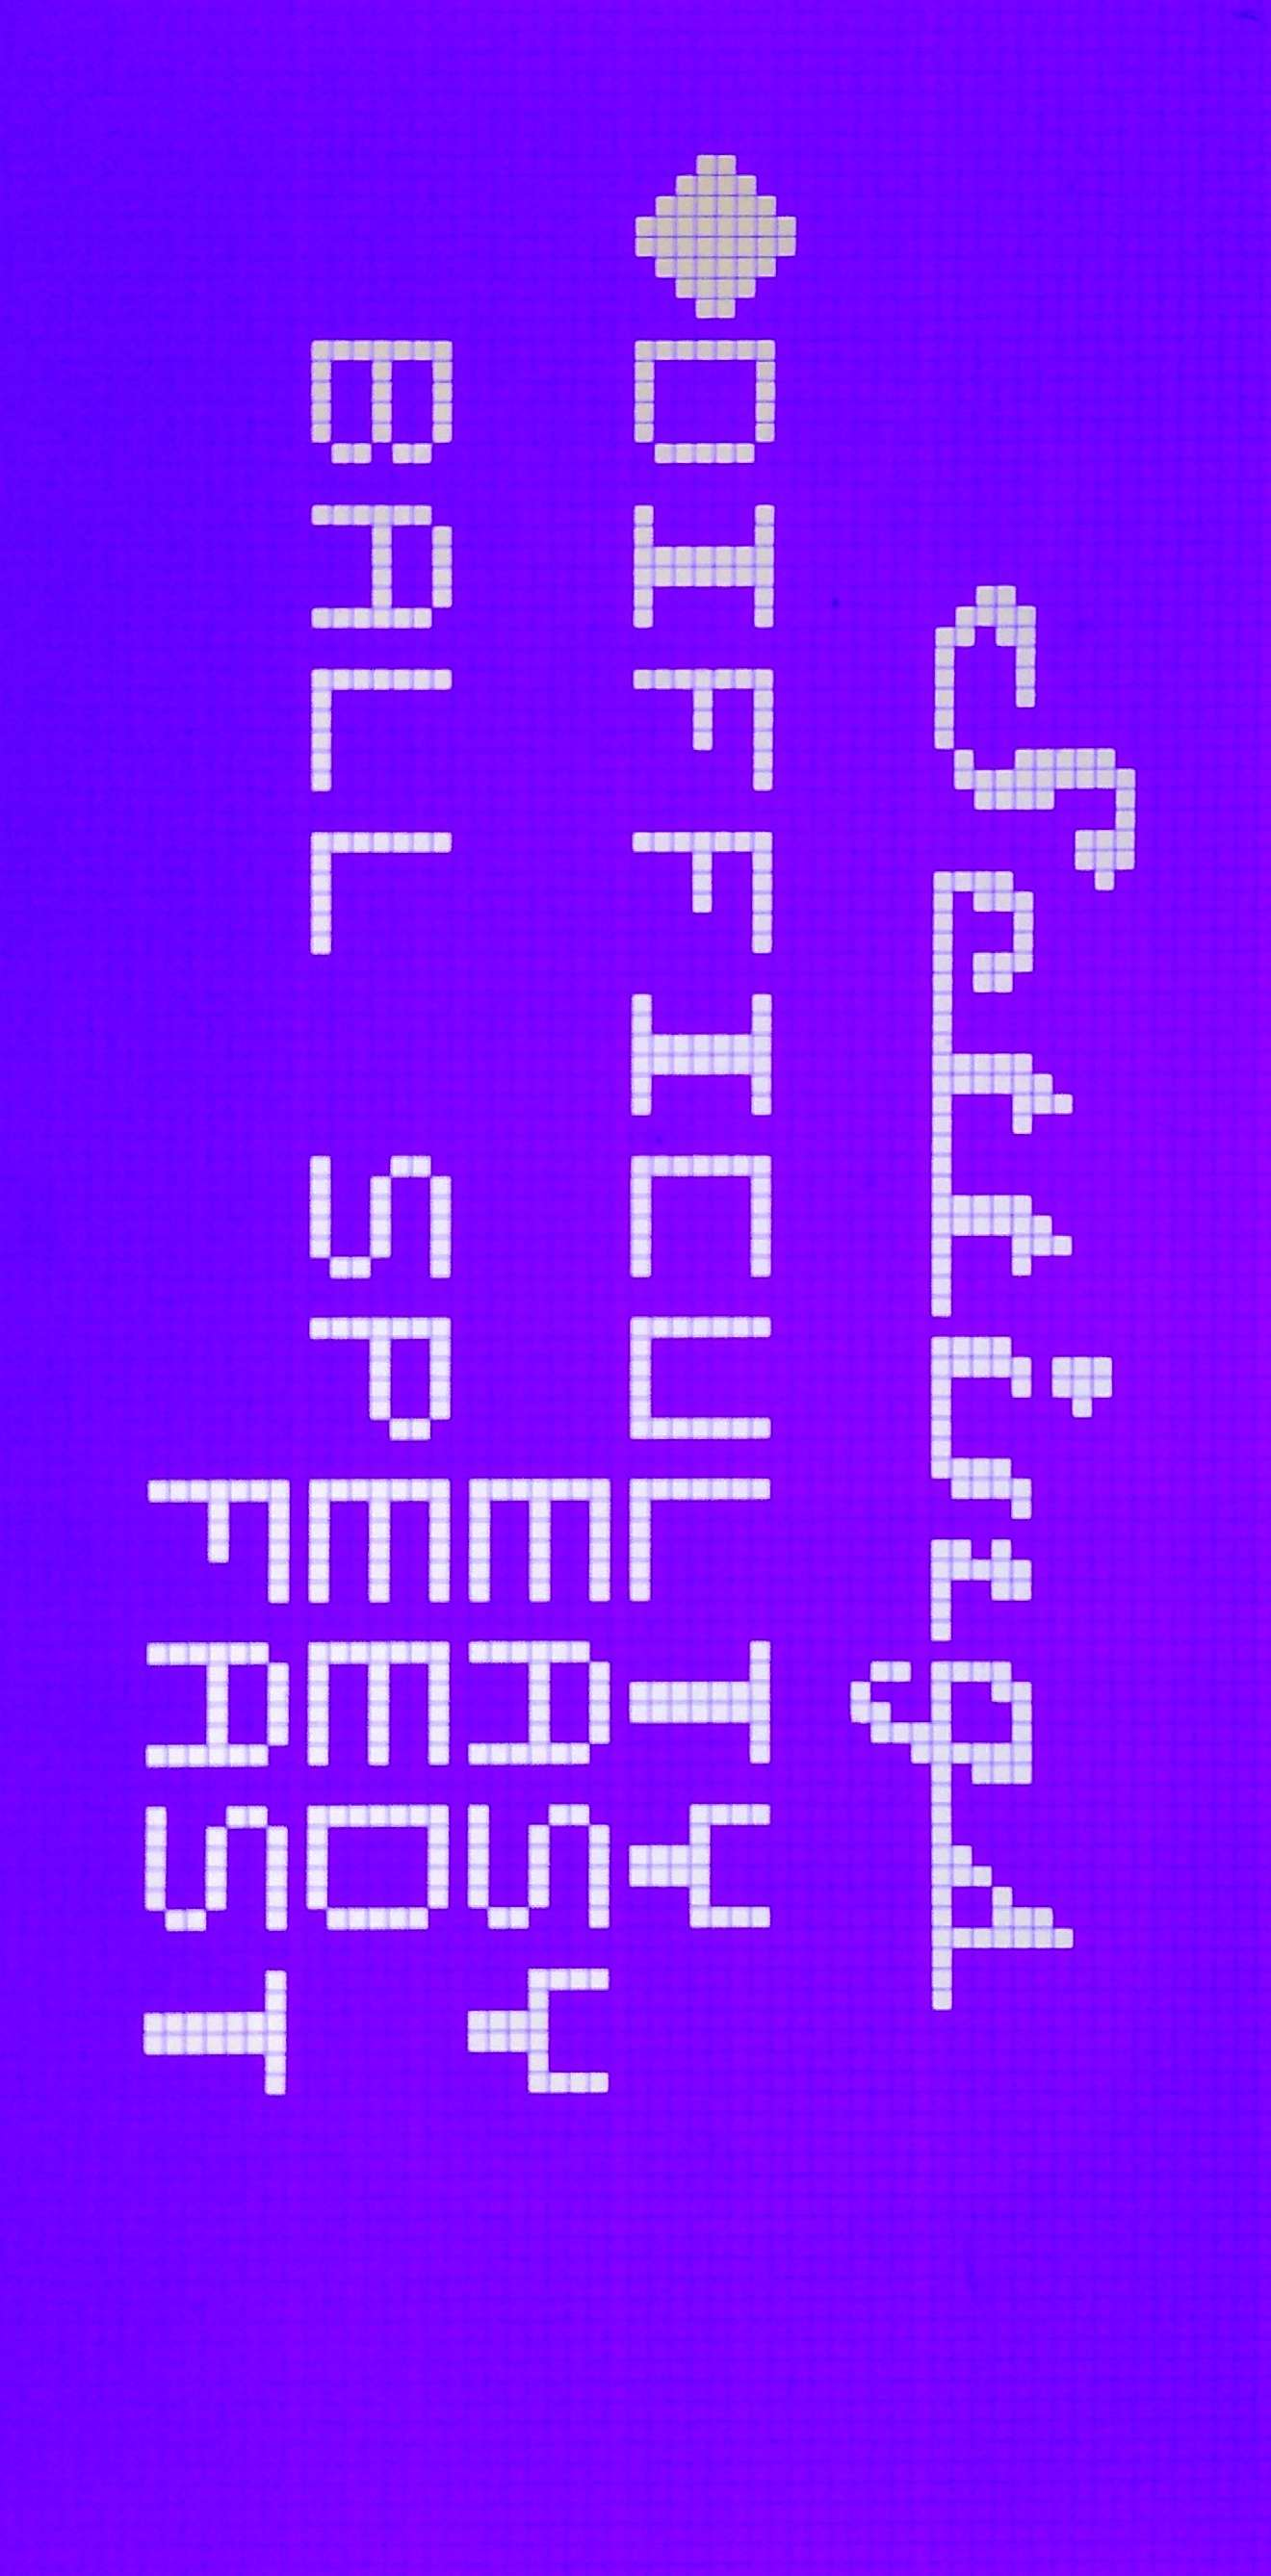
\includegraphics[width=5cm, height=10cm, angle = 90]{Images/settingsScreen} \\
  {\small Fig (d): Settings Screen} \\
  \end{center}
  \item \textbf{GAMEPLAY} State: \\ \qquad This is the actual gameplay screen running internal state machines.
  \\ Thumbstick moves paddle left or right.
  \\ The below screenshot shows a paddle at the bottom, a ball in transit in the \textit{UP LEFT} direction and certain bricks are removed.
  \begin{center}
  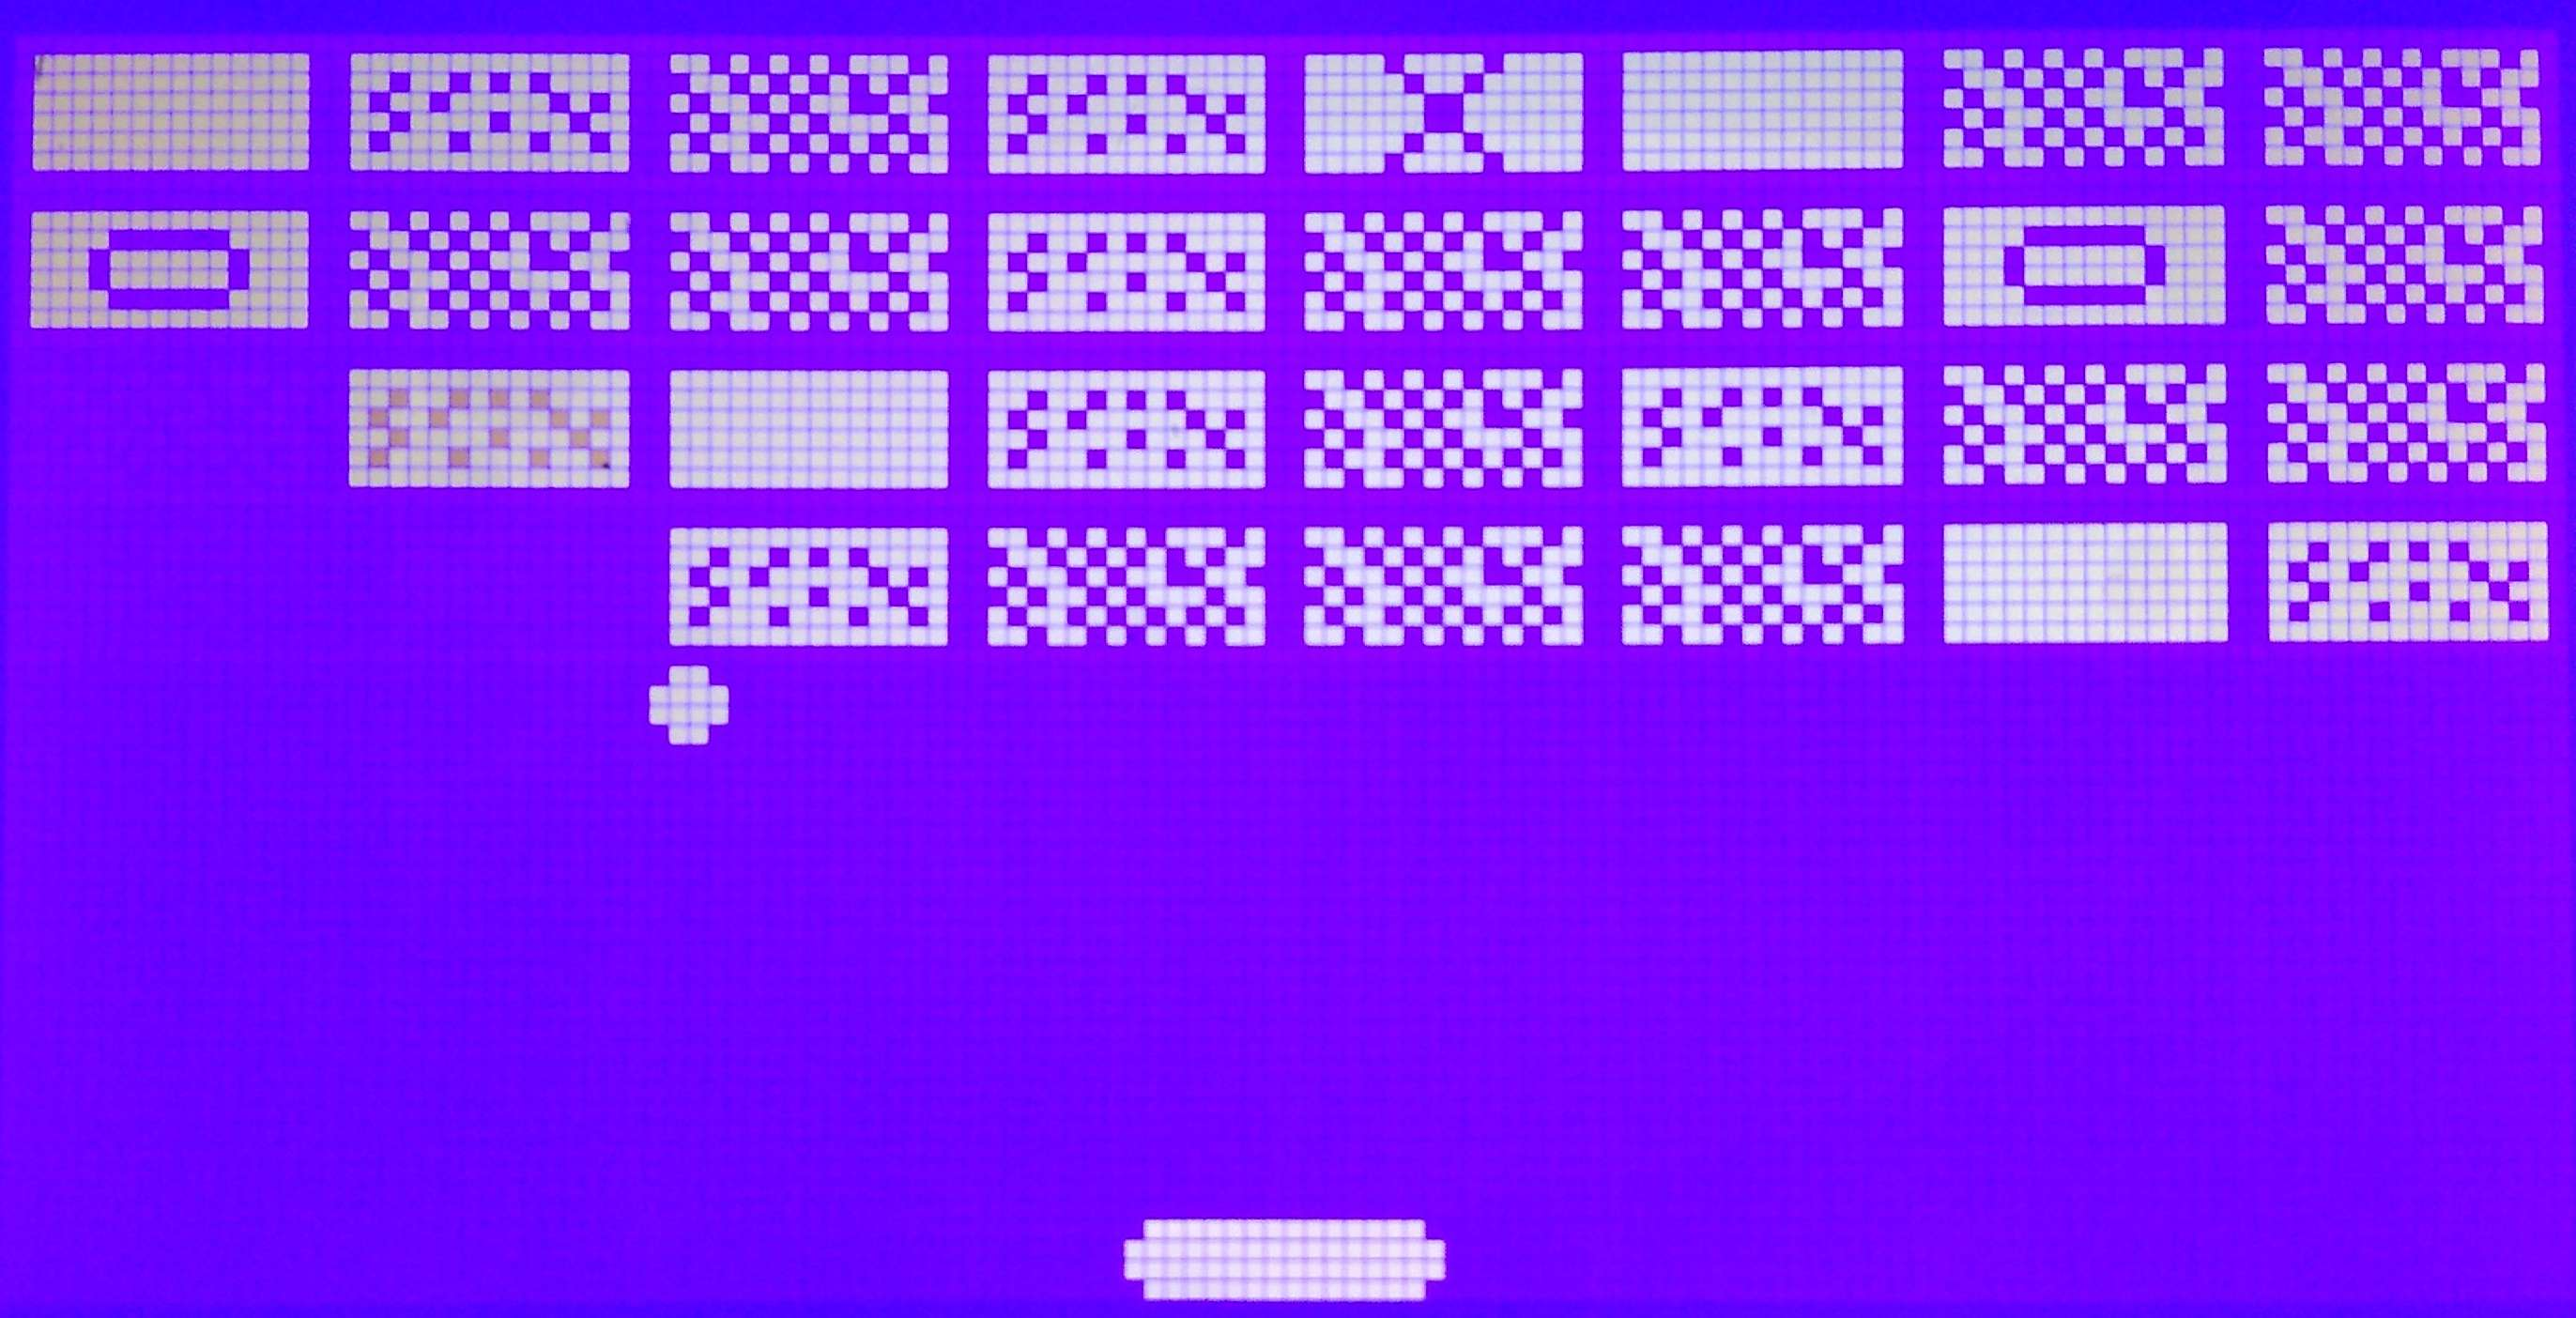
\includegraphics[width=10cm, height = 5cm]{Images/gameplayScreen} \\
  {\small Fig (e): Gameplay Screen} \\
  \end{center}
  \item \textbf{GAME OVER} State: \\ \qquad Once the player runs out of lives, the game over screen is displayed which accepts no input, but plays certain short music. Then returns to \textit{MENU} State.
  It can be as shown:
  \begin{center}
  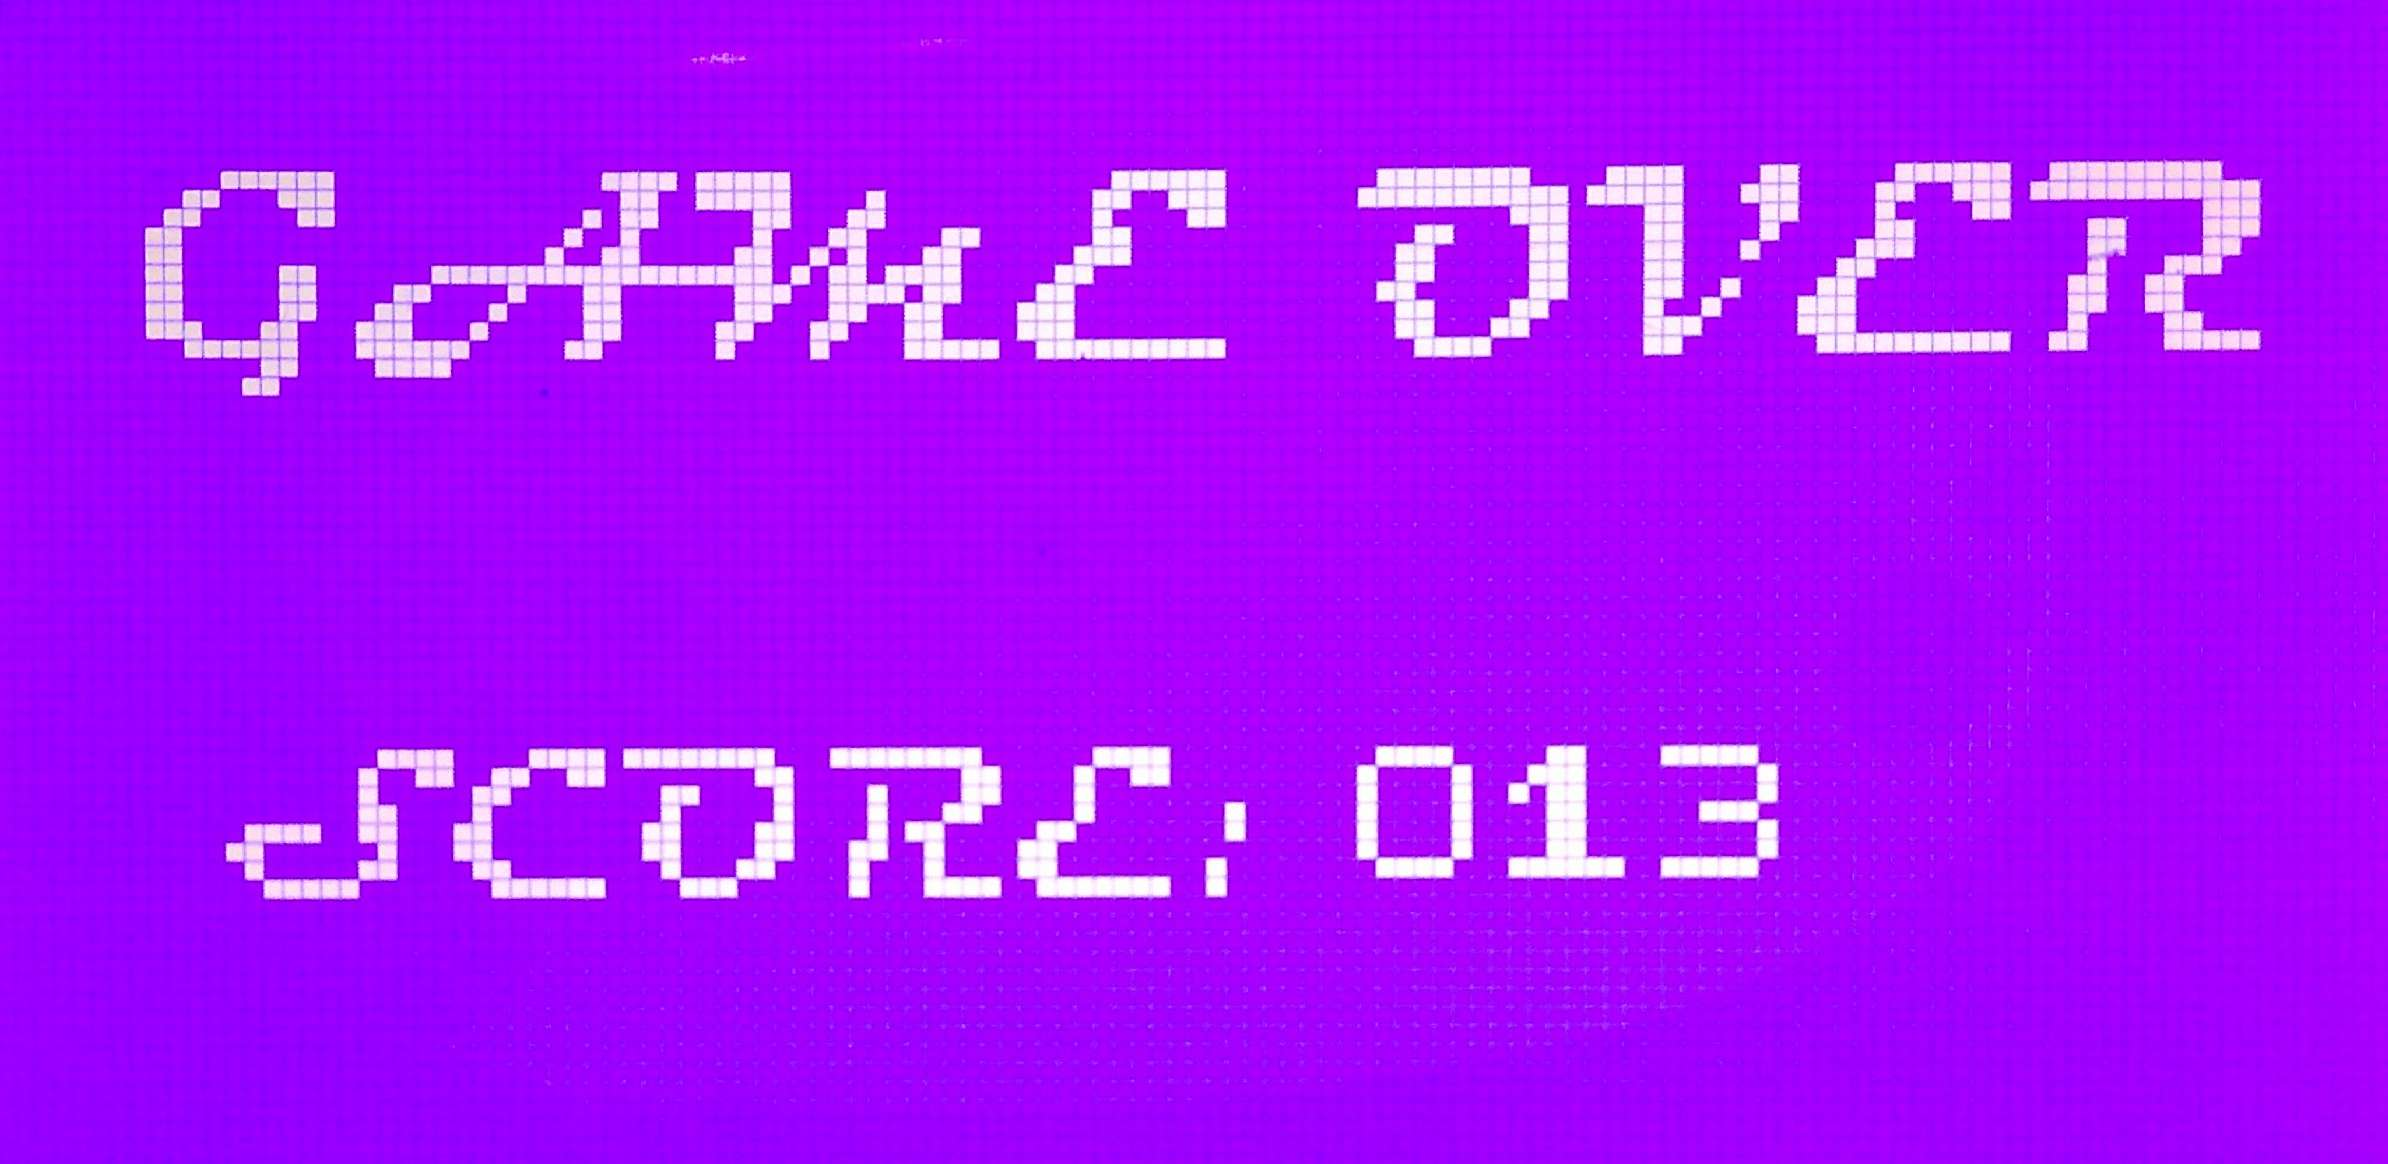
\includegraphics[width=10cm, height = 5cm]{Images/gameoverScreen} \\
  {\small Fig (f): Game Over Screen} \\
  \end{center}
  \item \textbf{VICTORY} State: \\ \qquad Once the player clears all bricks, a victory music is played over a victory screen, following end of music, game returns to \textit{MENU} State.
  \begin{center}
  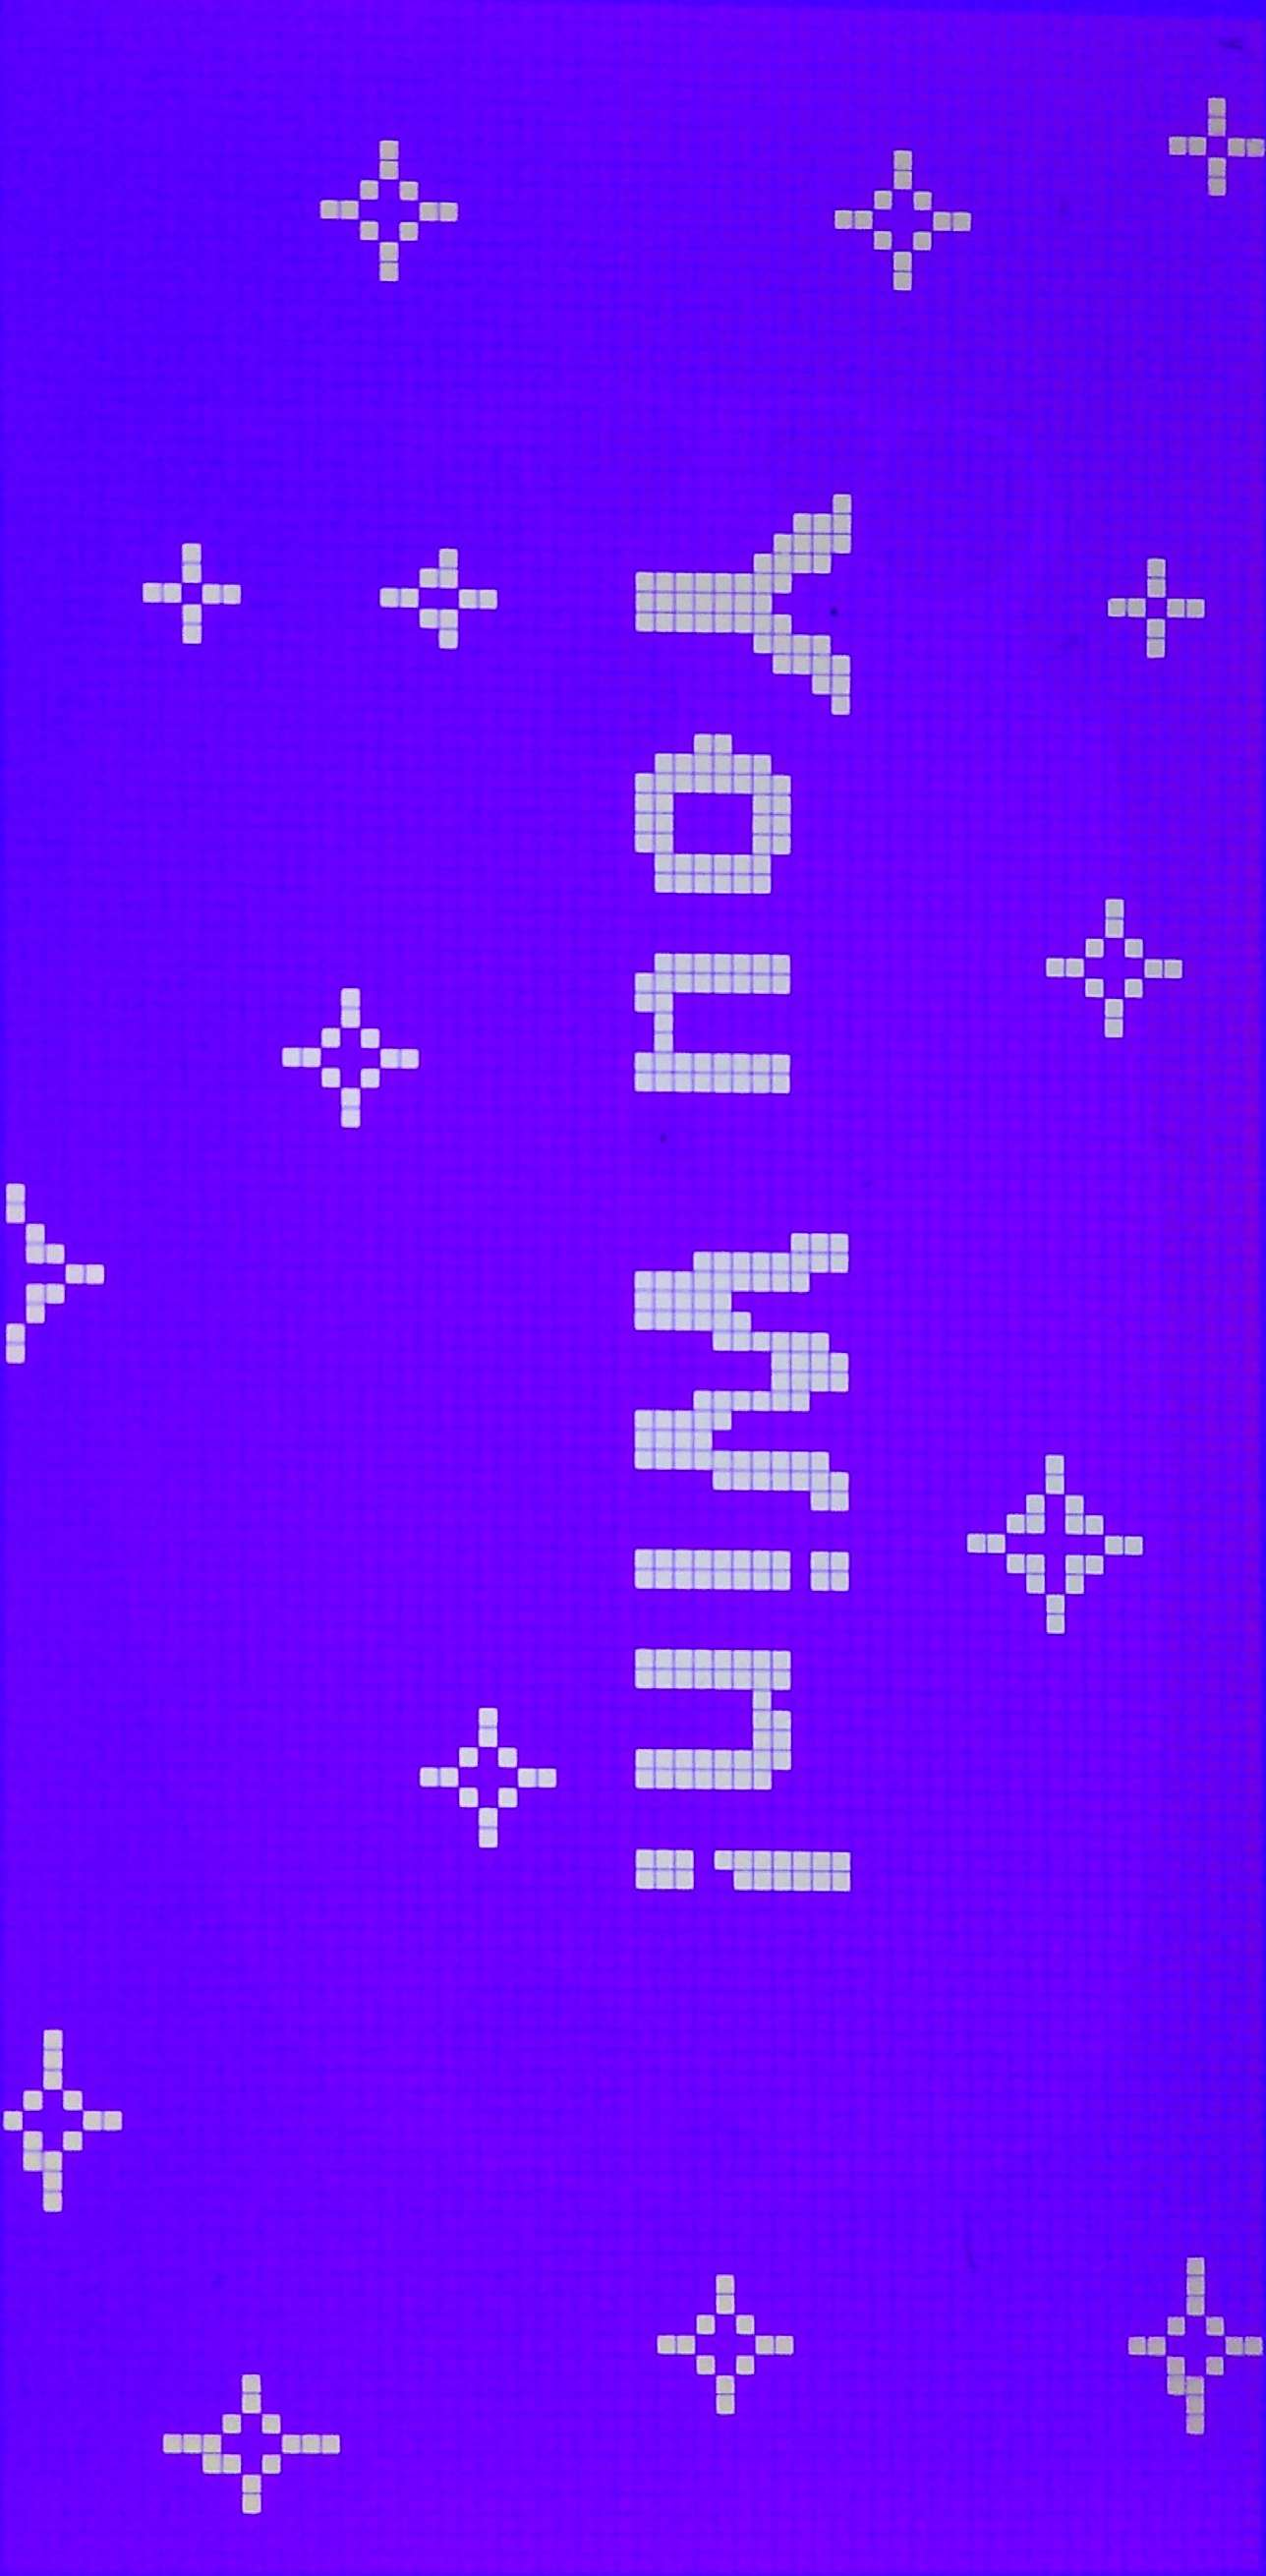
\includegraphics[width=5cm, height=10cm, angle = 90]{Images/victoryScreen} \\
  {\small Fig (g): Victory Screen} \\
  \end{center}
\end{itemize}
\begin{center}
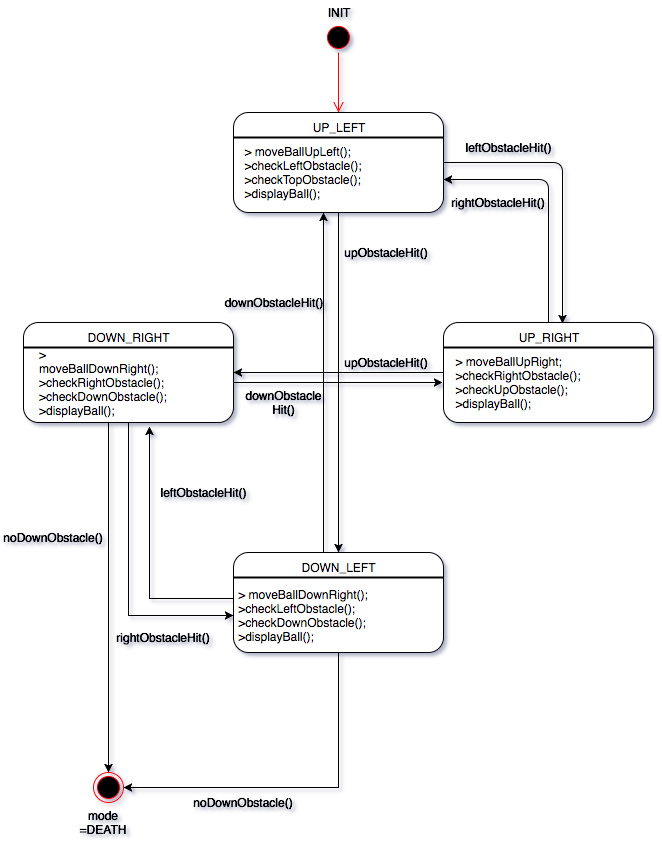
\includegraphics[width=14cm, height=16cm]{Images/ballDirectionStatemachine} \\
\caption{Fig (h): Ball Direction State Machine} \\
\end{center}
\qquad Fig (h) shows the various modes of motion of the ball. Unless an obstacle is detected, the ball continues to be in a particular state/ direction, as shown. If the obstacle is a brick, \textit{hit} variable is decremented. If an obstacle is not present at the bottom, a life is lost. If an obstacle is present at the bottom, it needs to be the paddle which is tracked with the ADC thumbstick input.
\begin{center}
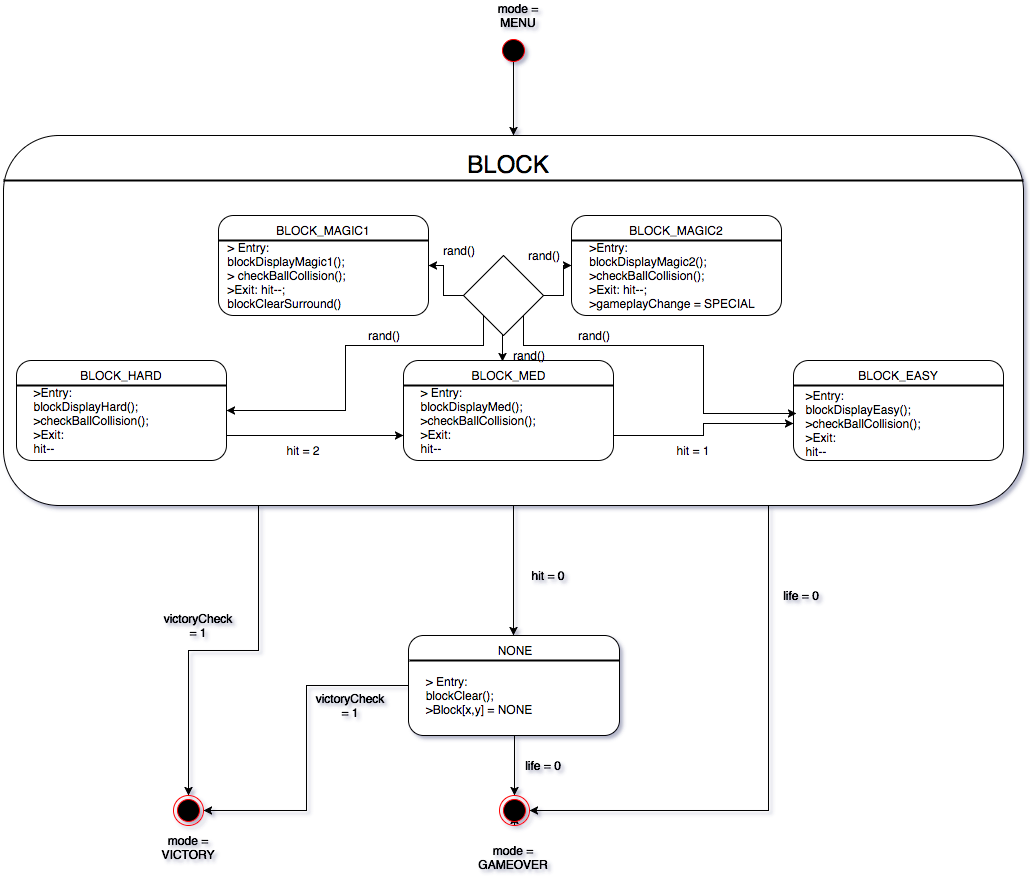
\includegraphics[width=14cm, height=14cm]{Images/brickTypeStatemachine} \\
\caption{Fig (i): Brick Type State Machine} \\
\end{center}
\qquad The above state machine denotes switching between various states of each block. Initially, a randomizer randomizes the entire block wall. Thereafter, based on ball hit, different blocks are eliminated. The brick state machine is terminated upon \textit{DEATH} and \textit{VICTORY}.
\begin{center}
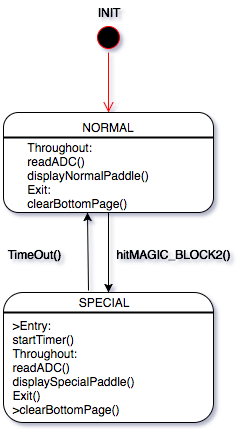
\includegraphics[width=4cm, height=7cm]{Images/paddleTypeStateMachine} \\
\caption{Fig (j): Paddle Type State Machine} \\
\end{center}
\qquad The visualization above represents the two different states for the paddle, the special extended state for 10 seconds once the ball hits BLOCK\_MAGIC2 and the normal state otherwise. Each state reads from ADC and displays the paddle at the appropriate position.
\begin{center}
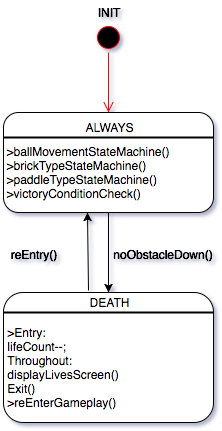
\includegraphics[width=4cm, height=7cm]{Images/gameplayStateMachine}\\
\caption{Fig (k): Gameplay Internal State Machine} \\
\end{center}
\qquad The above state machine shows two different states within gameplay. Gameplay continues till the player dies, upon which, certain tasks are performed.

 \subsection{RTOS Implementation}
 \qquad The Breakout Game can be implemented using two tasks: \textit{readInput()} and \textit{displayOutput()}
 \subsubsection{readInput() Task}
 \qquad Handles all input switch press detection and ADC thumbstick movement. The behaviour is different in different game screens, hence consists of an internal state machine which defines behaviour at different states, implemented using switch case.For example, \textit{SWITCH} press is an event in the \textit{MENU} state but not in the \textit{GAMEPLAY} state.
 \subsubsection{displayOutput() Task}
 \qquad Handles output screens to be displayed on GLCD corresponding to different states. Also handles LED outputs, Buzzer beeps and music, and also the vibration motor output. Hence different screens have different outputs, it consists of an internal state machine which determines the menu screen to be displayed in \textit{MENU} state, but Game over screen to be displayed, alongwith appropriate music in \textit{GAME OVER} state.
\section{Procedure}
\begin{enumerate}
\item \qquad Include all the relevant header files in your code. Ensure that the following header
files are present:
\begin{lstlisting}[basicstyle = \small, language = C]
#include "Console/consoleInit.h"
#include "Console/glcd.h"
#include "Console/gameDisplay.h"
#include "Console/tones.h"
#include "Objects/gameObjects.h"
#include "Screens/gameScreens.h"
\end{lstlisting}
\qquad The above libraries contain direct-to-GLCD font libraries, pre-made music and beeps, game graphic objects and screens in the form of accessible functions. The libraries can be downloaded from \href{https://github.com/eYSIP-2017/eYSIP-2017_Game_Development-TI-RTOS/blob/master/Documentation/Breakout/Console\%20Libraries.zip}{here}.
\item All necessary initialization, including Timers, Interrupts, Clock, ADC, GPIO, UART, etc. can be performed using function \_init\_() from consoleInit.h. Edit consoleInit.h to initialize other peripherals in addition to the ones provided.
\item Initialize each of the various states using enumeration as in the following example:
\begin{lstlisting}[basicstyle = \small, language = C]
enum modes
{
    /* Different game states(Classified because of 
    different I/O behaviour in each state) */
    MENU,
    INSTRUCTIONS,
    SETTINGS,
    GAMEPLAY,
    VICTORY,
    GAMEOVER
};
// Initialization
enum modes mode = MENU;
\end{lstlisting}
\item Declare two tasks(empty), with corresponding semaphores \textit{readInput()} and \textit{displayOutput()}.
\item Use Timer 2A Interrupt for task scheduling and post semaphores at appropriate instances in time.
\item Now, in each task, implement the overall game state machine, with its various internal state machines, as in the statecharts given in Section 4(Switch Case or State Table Implementation can be used).
\end{enumerate}
\section{Demo and Submission:}
\begin{itemize}
    \item Implement appropriate statechart within each task and use appropriate task scheduling in RTOS.
    \item Show working game demonstration to TA.
\end{itemize}
\begin{center}
\newline
   All The Best
  % \\[2\baselineskip]

 \end{center}
\end{document}
